\section{Parallelization Techniques}
\thispagestyle{plain}

Consider we can decompose a problem
into order-independent or partially-ordered
components of computation (\textit{concurrency})
then we can tap into the power of multiple
cores by parallel execution (\textit{parallelism}).

\subsection{Why do we need to parallelize?}
The most basic reason why we need parallelism is that we cannot arbitrarily
scale up sequential operations, the speed of a single core cannot be scaled
arbitrarily (very basically because logic gates have finite switching times
and otherwise problems of metastable states occur (oscillation
between states), because storage access has limited speed, because cooling becomes very difficult, ...) - 
\textcolor{green1}{we need to simultaneously work on parts of a problem}.

\note{To use parallelization the algorithm of interest must parallelize well, and necessary communication
between threads must be fast.}

Further scenarios where parallelization is advantageous are

\begin{itemize}
    \item In a big simulation, the data we want to process might not fit onto the memory
    of a single device.
    \item Different tasks might benefit from different hardware (e.g. complex instructions
    on the CPU, lots of simple instructions on the GPU).
\end{itemize}

\subsection{Hardware perspective and parallelism}
Computation is carried out on \textit{cores} which on the CPU receive the
data to process from a cache (where e.g. two cores might share a cache) which
in turn comes from a (random access) memory. The smallest unit of storage
transferred to a cache is a cache line, e.g. of $64$ \textbf{bytes} (a double
precision float has $64$ \textbf{bits} so $8$ bytes).

\subsubsection{We should write code reducing memory access | row and column major storing
convention for matrices}
The two possibilities for sequentially storing a matrix are \textit{row major}
and \textit{column major}, as illustrated in figure \ref{fig:row_col_major}.

\begin{figure}
    \centering
    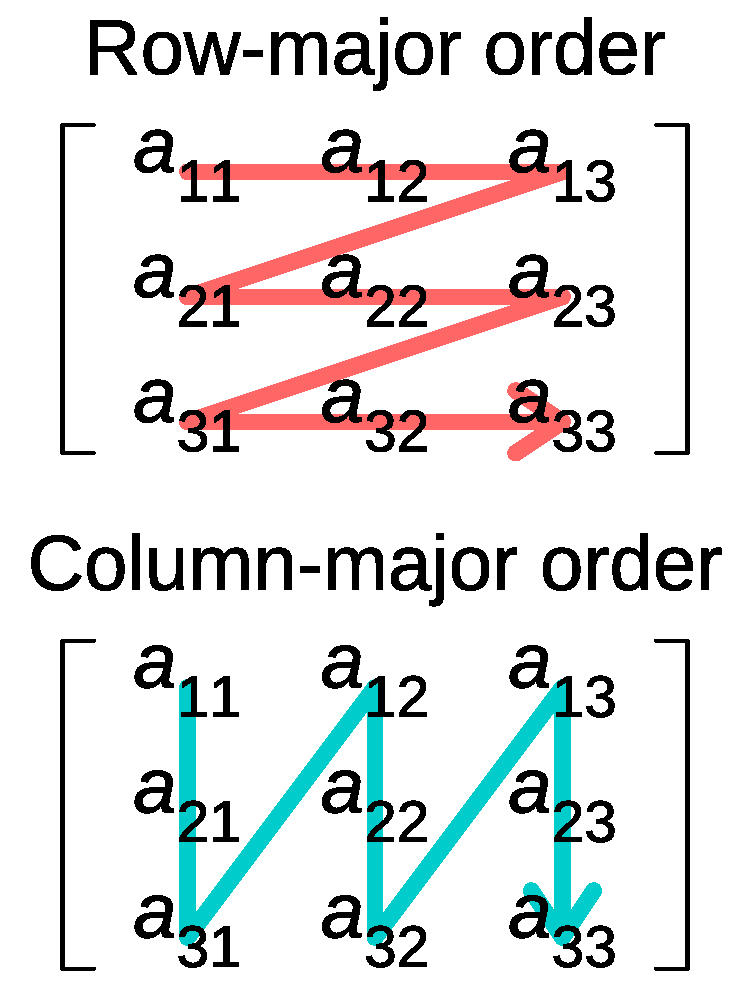
\includegraphics[width=0.4\textwidth]{figures/column_row.pdf}
    \caption{Row and column major storing convention for matrices.}
    \label{fig:row_col_major}
\end{figure}

As we transport full cache lines from the main storage, we have to optimize
our access according to the storage convention. E.g. in column major
one would do a matrix vector multiplication by addition of the scaled
column vectors.

\subsubsection{General computer architectures in increasing complexity\skipthis}

Architectures from serial to clusters can be found in table \ref{tab:architectures}.

\begin{table}
    \centering
    \begin{tabular}{|p{0.3\textwidth}|p{0.3\textwidth}|}
        \hline
        \textbf{Architecture} & \textbf{Characteristics} \\
        \hline
        Serial computer & The central processing unit (CPU) executes a single stream (of load, compute, store operations), one operation at a time \\
        \hline
        Multi core nodes & Multiple cores are connected to a single memory and can execute operations simultaneously \\
        \hline
        Multi-socket computing nodes & Each multi-core CPU preferably accesses its memory bank but all cores can access the full memory (but not everything at the same speed) \\
        \hline
        Compute Clusters & Many computing nodes are connected via a communication network (Infiniband better than Ethernet) \\
        \hline
    \end{tabular}
    \caption{General computer architectures in increasing complexity.}
    \label{tab:architectures}
\end{table}

\subsubsection{CPU vs GPU}
GPUs are specialized for executing many floating point operations in parallel. CPUs and GPUs
are used complementarily to have the speed in floating point operations of the GPU and the
complex instructions of the CPU.

CPUs and GPUs use Arithmetic Logical Units (ALUs) for the basic operations.

CPUs and GPUs are compared in table \ref{tab:cpu_gpu} and figure \ref{fig:cpu_gpu}.

\begin{figure}
    \centering
    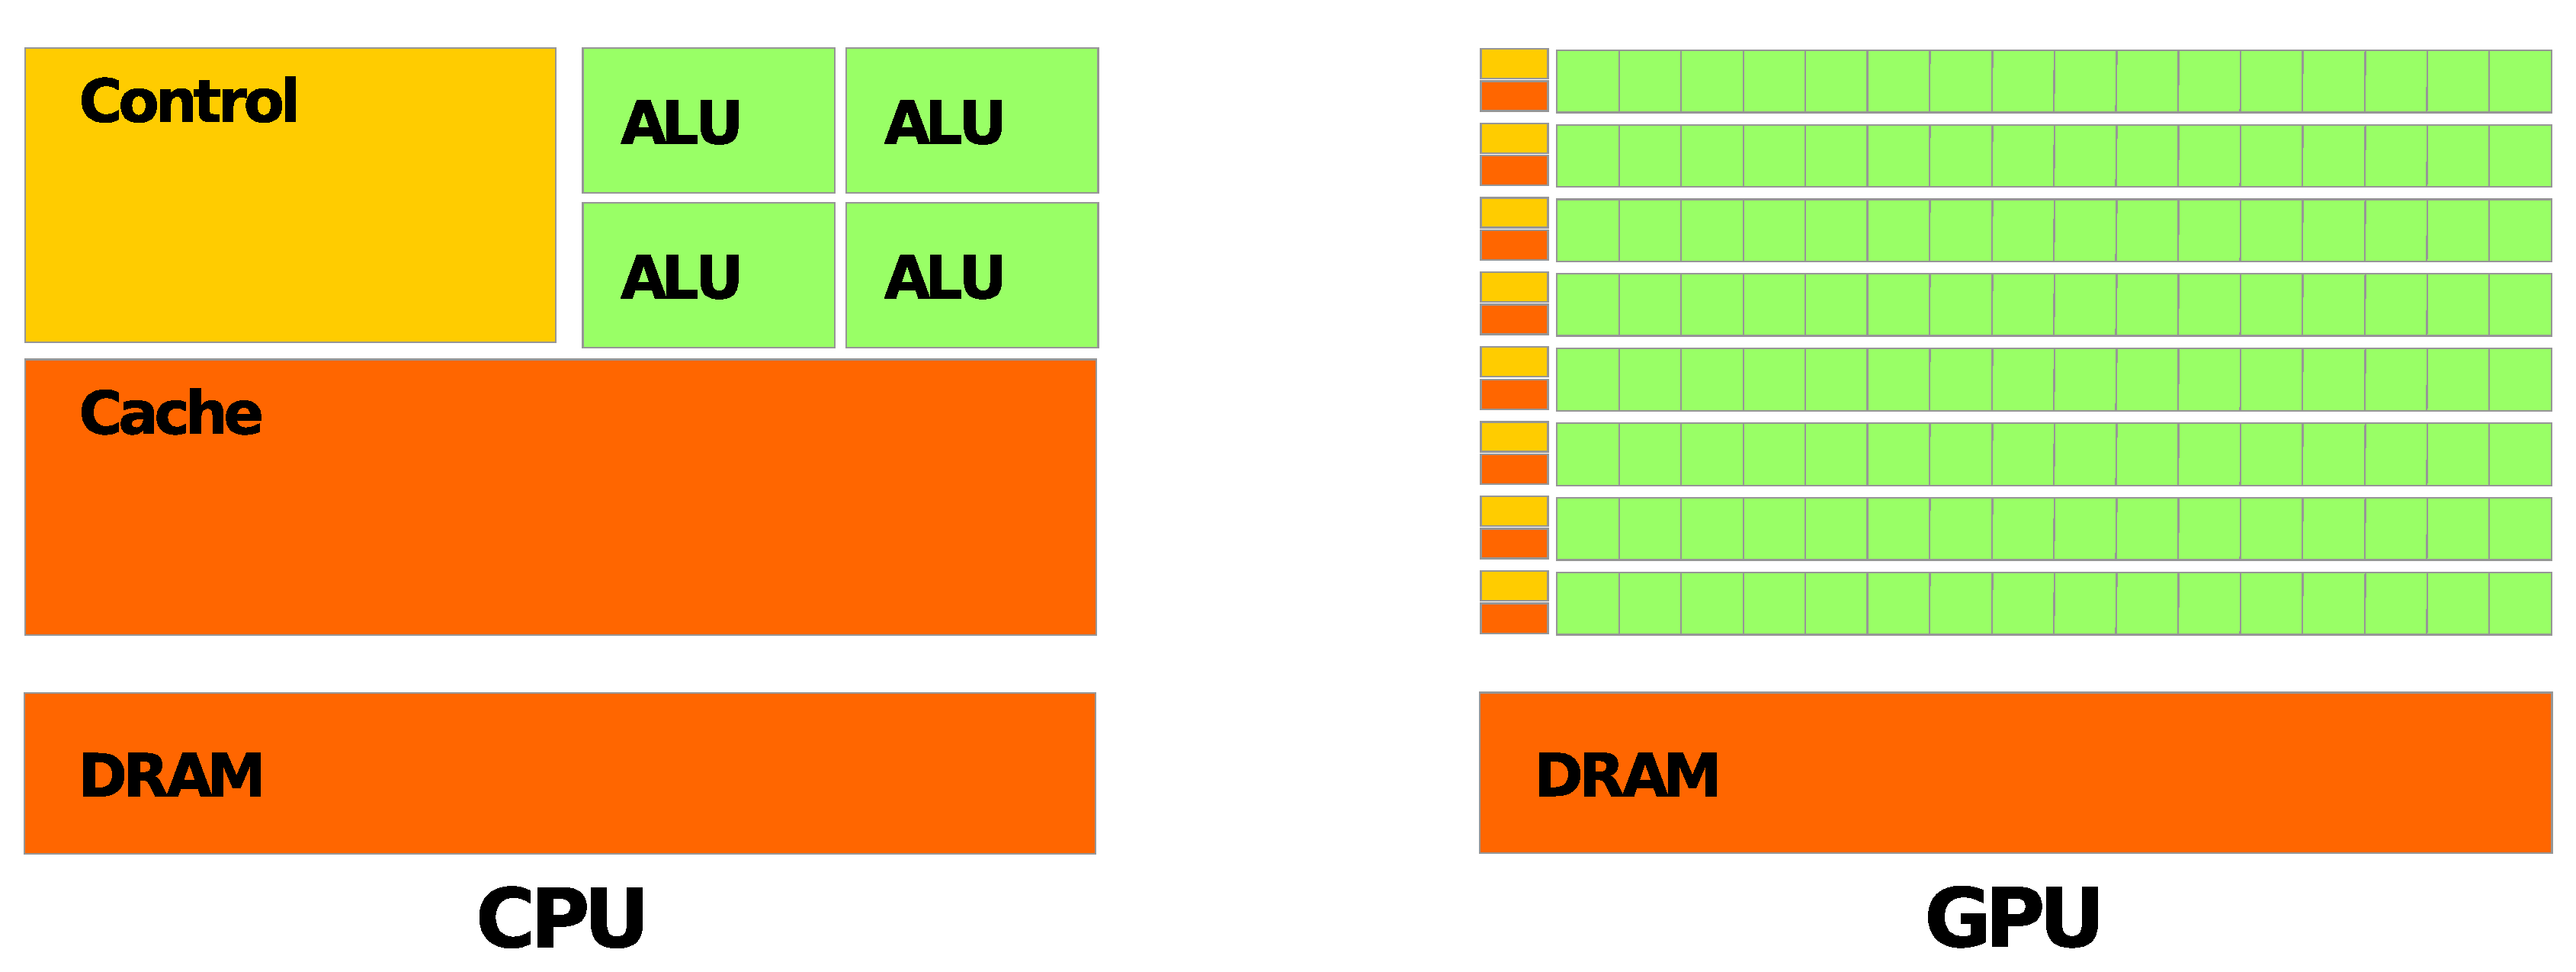
\includegraphics[width=0.6\textwidth]{figures/cpu_gpu.pdf}
    \caption{GPUs are build for parallel operations over many ALUs, CPUs for more complex operations over fewer ALUs.}
    \label{fig:cpu_gpu}
\end{figure}

\begin{table}
    \centering
    \begin{tabular}{|p{0.45\textwidth}|p{0.45\textwidth}|}
        \hline
        \textbf{CPU} & \textbf{GPU} \\
        \hline
        Optimized for serial operations
        \begin{itemize}
            \item few ALUs ($4$ to $16$)
            \item high clock speed ($\sim 3$ GHz)
        \end{itemize} & Optimized for parallel operations
        \begin{itemize}
            \item many ALUs ($1000$s)
            \item lower clock speed ($\sim 1.5$ to $2$ GHz)
        \end{itemize} \\
        \hline
        \begin{itemize}
            \item each core runs its own code
            \item complex control logic $\rightarrow$ general purpose
            \item shallow instruction pipelines\tablefootnote{Instruction pipelining is a technique for implementing instruction-level parallelism within a single processor.}
        \end{itemize} & \begin{itemize}
            \item many cores run the same code
            \item simple control logic $\rightarrow$ specialized for parallel operations
            \item deep instruction pipelines
        \end{itemize} \\
        \hline
        \begin{itemize}
            \item low compute density (?)
            \item large but slow memory
            \item faster data transfer
        \end{itemize} & \begin{itemize}
            \item high compute density
            \item high computation per mean access
            \item slower data transfer
        \end{itemize} \\
        \hline
    \end{tabular}
    \caption{Comparison of CPUs and GPUs.}
    \label{tab:cpu_gpu}
\end{table}

\subsubsubsection{When and how to use GPUs}
As data transfer to the GPU is slower
\begin{itemize}
    \item copy data rarely / copy little data
    \item run the same code on all cores
    \item run many instructions
\end{itemize}
e.g. for
\begin{itemize}
    \item $N^2$ force terms in direct summation
    \item (blocked) matrix multiplication
    \item ...
\end{itemize}

\subsubsection{Vector cores}
Many single compute cores can carry out vector instructions, i.e. apply one operation
like addition to multiple elements (a vector).

\subsubsection{Hyperthreading}
At some point speed is more limited by the slow data transfer from memory 
to the cores than the speed of the cores. In hyperthreading, waiting time is 
efficiently used - we overload the computation core with execution streams and 
switch rapidly between these hyperthreads so we can use waiting time efficiently. 
This way we effectively have more “virtual cores” than physical ones.

\subsection{Types and challenges of concurrency and parallelism}
\subsubsection{Shared memory and message passing concurrency}
The basic question is, how processes can be coordinated.
Shared memory and message passing concurrency are compared in table \ref{tab:shared_message}.

\begin{table}[!htb]
    \centering
    \begin{tabular}{|p{0.45\textwidth}|p{0.45\textwidth}|}
        \hline
        \textbf{Shared memory} & \textbf{Message passing} \\
        \hline
        \begin{itemize}
            \item processes coordinate by reading and writing 
            to shared memory locations
            \item locks are used to manage concurrent access
            to memory (or on a higher level a sophisticated
            type system as Rusts ownership system avoiding race
            conditions automatically)
        \end{itemize} & \begin{itemize}
            \item processes coordinate by sending and receiving messages through channels
            \item channel operations need to be managed
            \item process results can e.g. be brought together at barriers
        \end{itemize} \\
        \hline
        \begin{itemize}
            \item OpenMP in C
            \item Threads in Rust
        \end{itemize} & \begin{itemize}
            \item MPI in C
            \item Go-routines combined with channels in Go, \textit{sharing memory by communicating instead of communicating by sharing memory}
        \end{itemize} \\
        \hline
    \end{tabular}
    \caption{Comparison of shared memory and message passing concurrency.}
    \label{tab:shared_message}
\end{table}

\greenbox{Based on message passing concurrency we can have distributed memory parallelization, where our program can run on multiple computers.}

\subsubsection{Challenges of concurrency}
\begin{itemize}
    \item \textcolor{red1}{Race conditions in shared memory concurrency}: if 
    different threads can modify the same variable at the same time, bugs can 
    quickly arise or even memory corruption
    \item \textcolor{red1}{Deadlocks}: being stuck forever aquiring a lock in shared memory concurrency (cyclic waiting)
    or waiting for a message that never arrives or never being able to send to a channel in message passing concurrency
    \item \textcolor{red1}{Livelock}: repeating the same interaction without doing useful work
\end{itemize}
Note that for instance in the message passing model, by adequate types of channels
(protocols specifying the usage of the channel (e.g. first send, then receive)) where for a
\textit{linearly typed channel} every capability must be used exactly once and only using
dual pairs of channels (e.g. dual of the previous example: first receive then send) deadlock freedom can be guaranteed.

\subsection{Shared memory parallelization (with OpenMP)}
In shared memory parallelization, work is distributed to threads with access to the same memory.
\redbox{Shared memory parallelization is limited to one node / CPU.}

In C/C++/Fortran, OpenMP is a language / compiler extension for shared memory parallelization.

\subsubsection{Simplest parallelization - parallel for loop of independent iterations}
If order does not matter, we can simply parallelize a for loop as done in code \ref{code:parallel_for}.

\begin{codebox}[!htb]
    \begin{minted}{cpp}
        #pragma omp parallel for
        for (int i = 0; i < N; i++) {
            some_expensive_calculation(i);
        }
    \end{minted}
    \caption{Loop parallelization with OpenMP.}
    \label{code:parallel_for}
\end{codebox}


\subsubsection{OpenMP's fork-join model}
Sections of the code are run in parallel (starting from the main thread) and joined again.
This is illustrated in figure \ref{fig:fork_join}.

\begin{figure}[!htb]
    \centering
    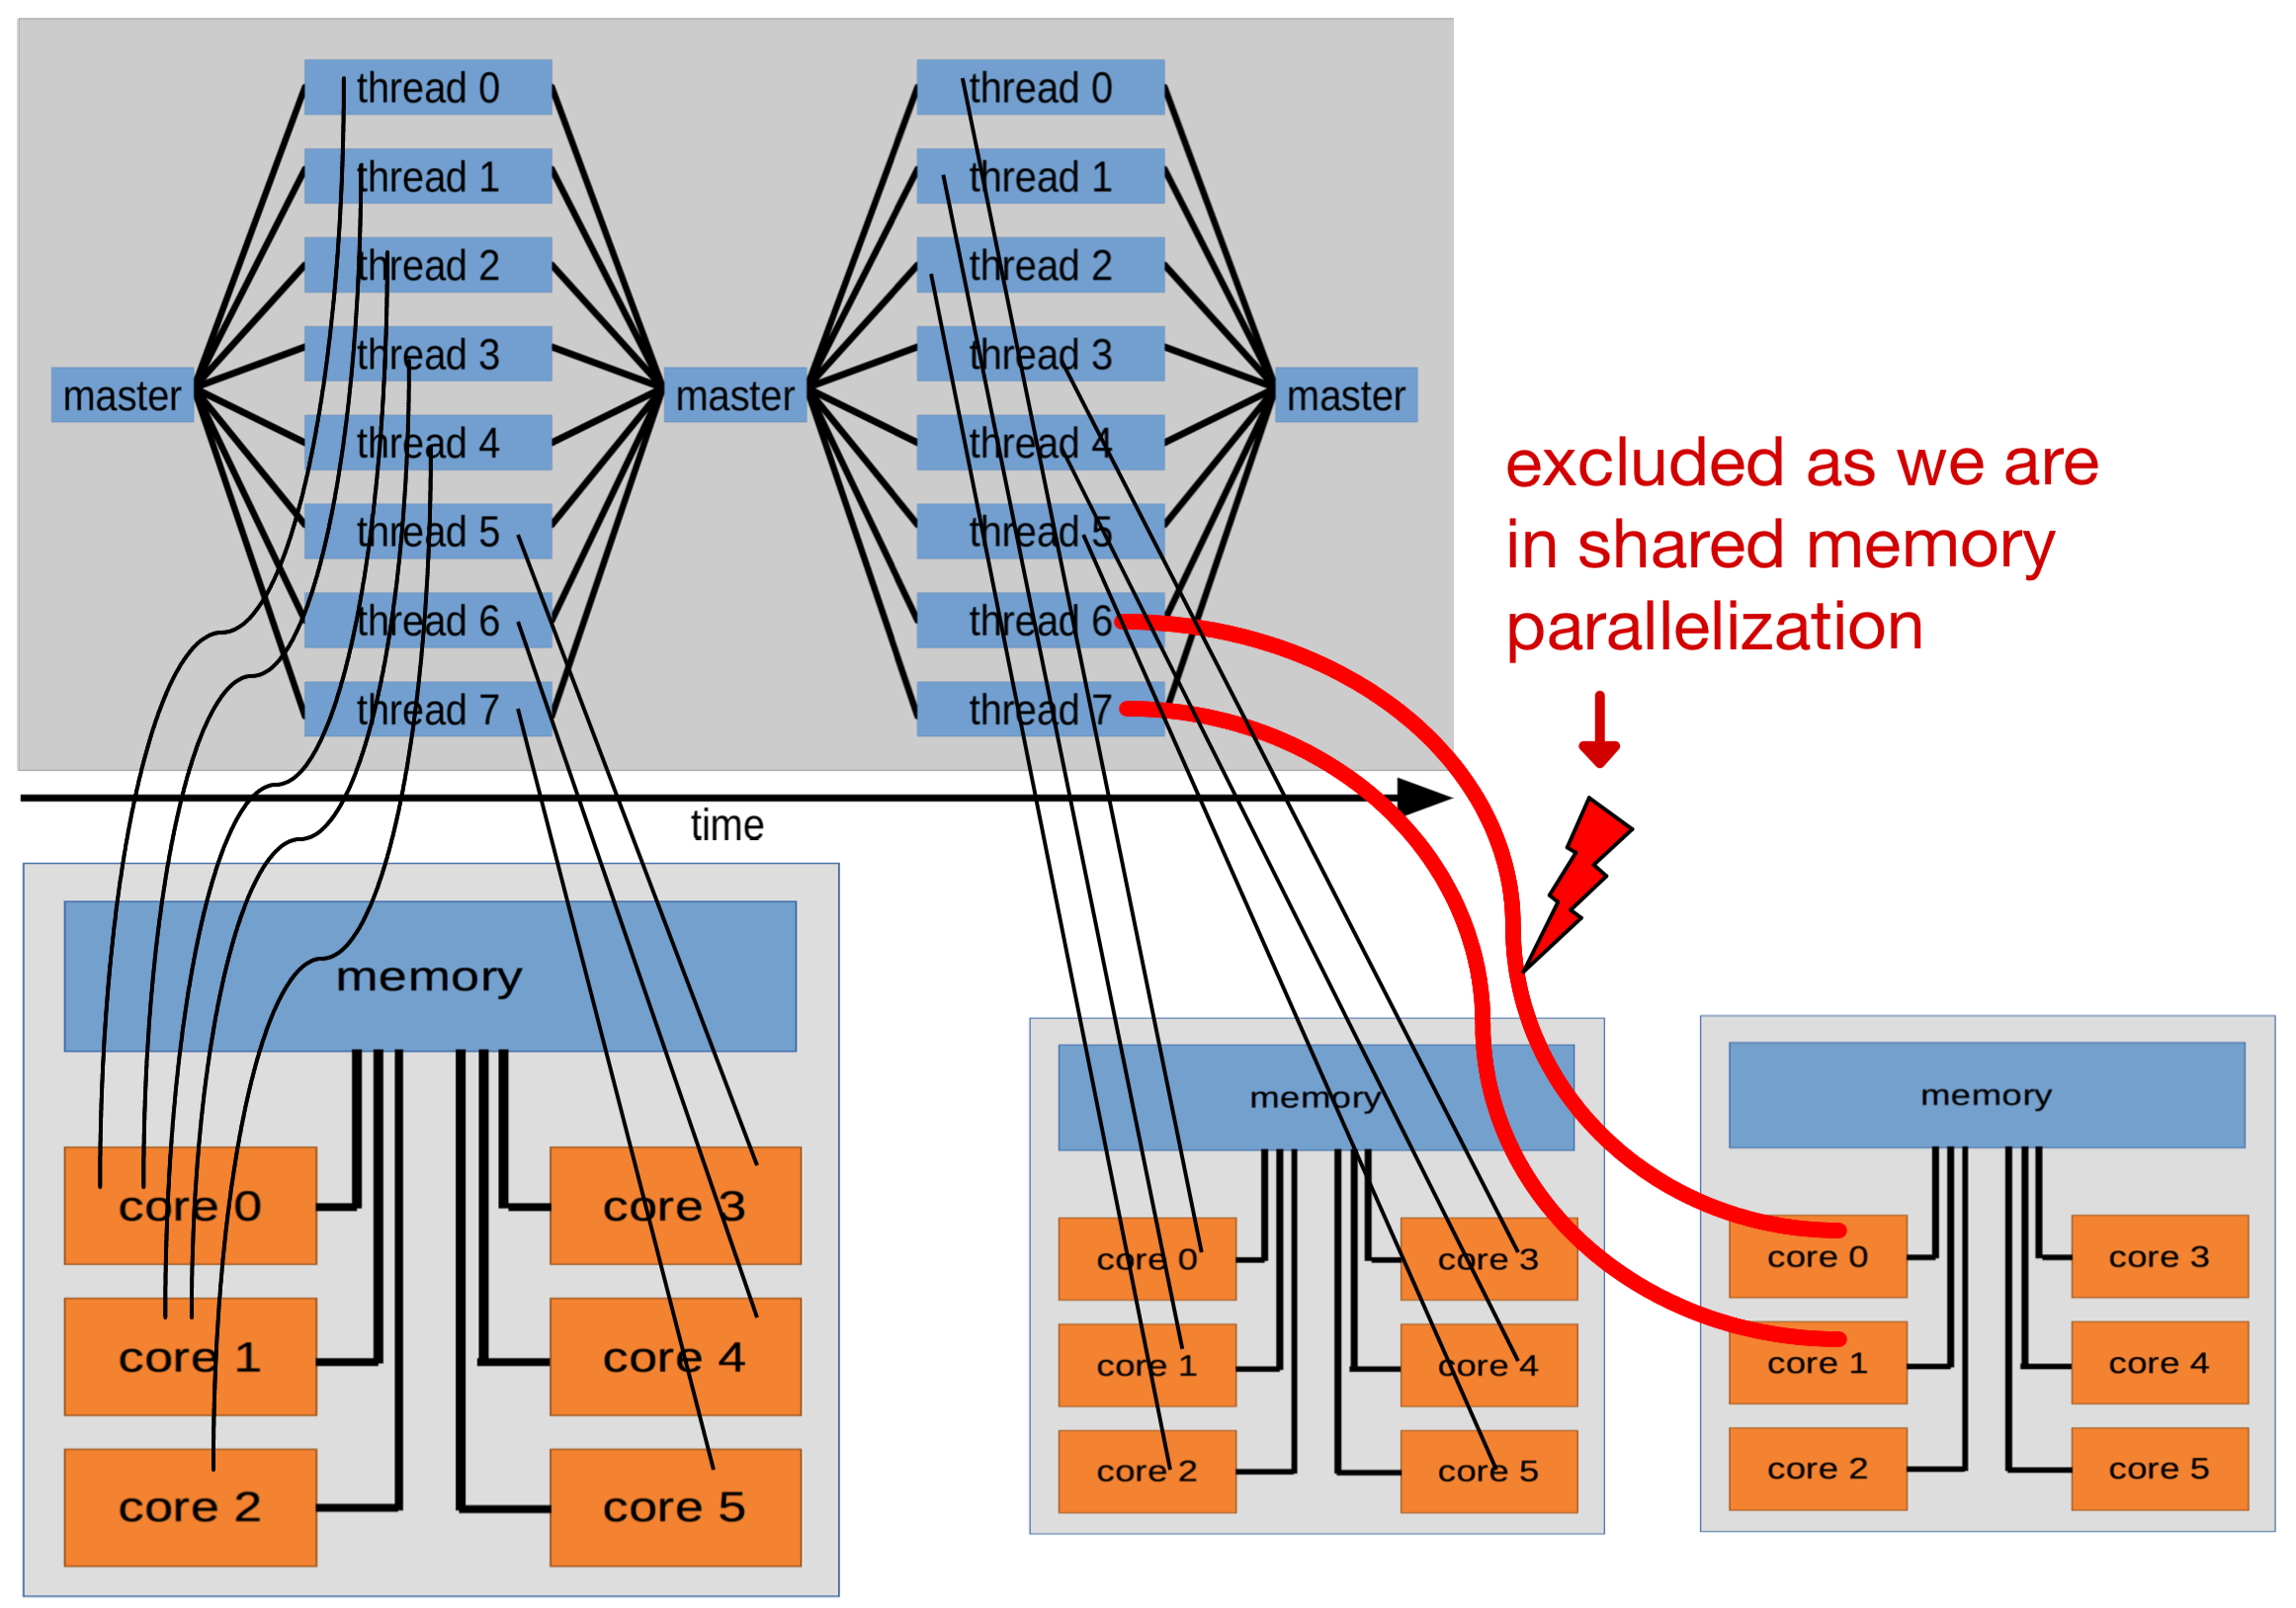
\includegraphics[width=0.8\textwidth]{figures/fork_join.png}
    \caption{OpenMP's fork-join model.}
    \label{fig:fork_join}
\end{figure}

\subsubsection{Race conditions}
If different threads can modify the same variable at the same time, bugs can quickly arise.
\subsubsubsection{Race conditions in the context of non-atomic operations}
An operation like \texttt{a = a + 1} is not atomic, but actually three operations:
\begin{itemize}
    \item read the value of \texttt{a}
    \item add $1$
    \item write the new value to \texttt{a}
\end{itemize}
In a setting where one thread might read before another thread has written, we get into trouble,
as illustrated in go in code \ref{code:parallel_counter_go} and in C in code \ref{code:parallel_counter_c}.
\bluebox{To avoid races, critical areas can be defined, that can only be accessed by one thread at a time, all others have to wait.
\textcolor{red1}{This also adds a bottleneck to parallelization}. A more fine-tuned approach is to lock memory, not code,
where there can be multiple reads at the same time, but writes exclude all other operations.}

\begin{codebox}[!htb]
    \begin{minted}{go}
        func add_one(x *int) {
            *x = *x + 1 // really three instructions
            // 1. dereference pointer, 2. add 1, 3. assign to x
        }
        
        func main() {
            x := 0
            for i := 0; i < 1000; i++ {
                go add_one(&x)
            }
            time.Sleep(2 * time.Second)
            println(x) // e.g. 990
        }        
    \end{minted}
    \caption{Parallel counter in Go. As a solution one could use a lock, or an addition worker with
    an input channel on which numbers are sent, and an input channel on which channels are sent
    on which the current value of the counter is sent back.}
    \label{code:parallel_counter_go}
\end{codebox}

\begin{codebox}[!htb]
    \begin{minted}{cpp}
        int count = 0;
        // faulty addition
        #pragma omp parallel for
        for (int i = 0; i < 1000; i++) {
            for (int j = 0; j < 1000; j++) {
                count++;
            }
        }
        // correct e.g. by defining a critical area, so
        // ...
        #pragma omp critical
        {
            count++;
        }
        // ...
        // or by the annotation
        #pragmo omp parallel for reduction(+:count)
        // loop as before
    \end{minted}
    \caption{Parallel counter in C.}
    \label{code:parallel_counter_c}
\end{codebox}

\subsubsection{Using the same variable where it is not intended}
\problem{In code \ref{code:double_loop}, j is used in all loops over i, so the inner loops
interfere.}
\greenbox{\textbf{Solution:} Give each thread its own j.}
Another example in go is given in code \ref{code:same_var_go}.

\begin{codebox}[!htb]
    \begin{minted}{cpp}
        #pragma omp parallel for private(j)
        // without private(j) the inner loops interfere
        for (int i = 0; i < N; i++) {
            for (int j = 0; j < N; j++) {
                // do something
            }
        }
        
    \end{minted}
    \caption{Problem with using the same variable where it is not intended.}
    \label{code:double_loop}
\end{codebox}

\begin{codebox}[!htb]
    \begin{minted}{go}
        var wg sync.WaitGroup
        wg.Add(5)
        for i := 0; i < 5; i++ {
            go func() {
                println(i) // race on i!
                // when goroutine reads i
                // its already incremented
                wg.Done()
            }()
        }
        wg.Wait()
        // output e.g.: 2 5 5 5 5
        // solution, pass i as argument
    \end{minted}
    \caption{Races can be devious.}
    \label{code:same_var_go}
\end{codebox}

\subsection{Message passing concurrency enabling distributed memory parallelization (with MPI)}
In message passing concurrency threads communicate by messages rather than by access to the same memory.
In a message passing concurrency setting, different processes can be on different nodes and be executed
individually with their own (part of) memory.

\textbf{Example:} All nodes might run the same code for a physical simulation
but with different data (e.g. different parts of the grid) (single program,
multiple data (SPMD)).

\note{OpenMP and MPI can be used together, e.g. OpenMP on each node and MPI for communication between nodes.}

\subsubsection{Architecture of an MPI program}
The basic modes of communication in MPI are individual communication between two processes and collective communication.
At barriers, results are brought together, the scheme is illustrated in figure \ref{fig:mpi_architecture}.
\bluebox{A different approach is using channels onto which messages are sent and drawn from where the threads
are shared between the channels (as in Go). We can for instance realize a worker pool where there are different
worker threads drawing from a channel on which tasks are sent. Or pipelines ...}

\begin{figure}[!htb]
    \centering
    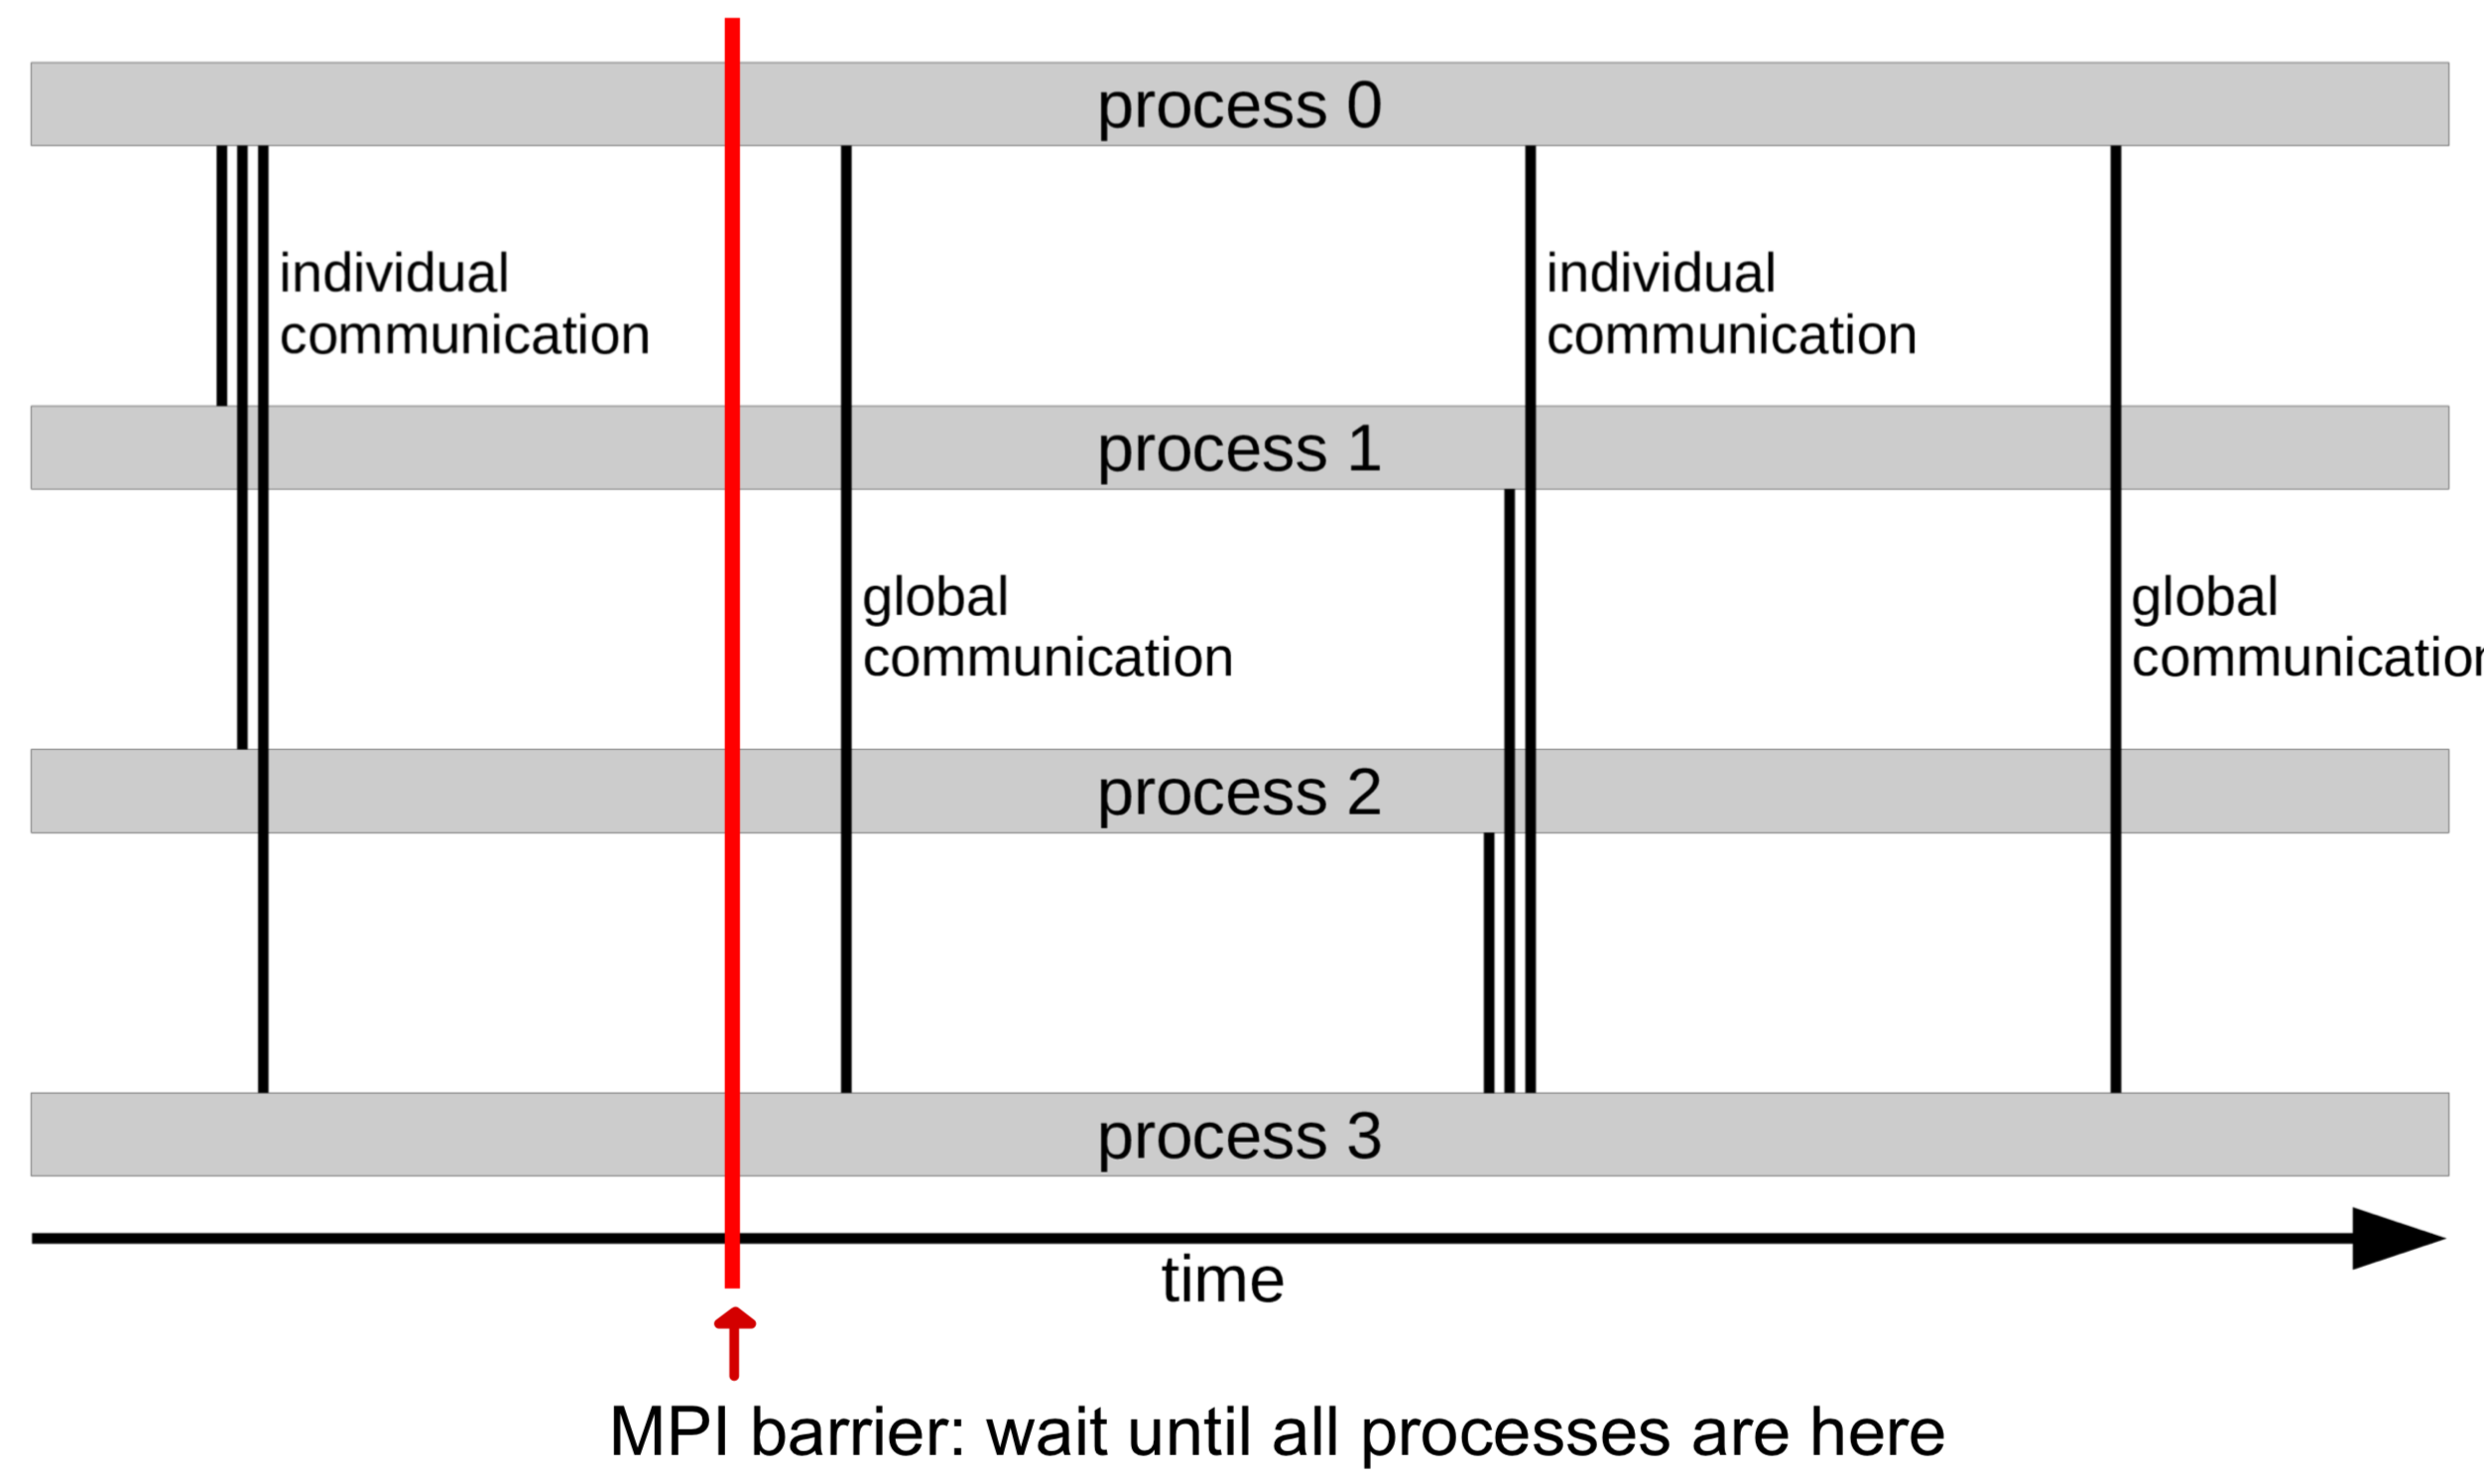
\includegraphics[width=0.8\textwidth]{figures/mpi_architecture.png}
    \caption{Architecture of an MPI program.}
    \label{fig:mpi_architecture}
\end{figure}

\subsubsection{MPI program structure and basic communication}
The basic idea is to start multiple instances of a program, where different instances
can have different behavior based on their uniquely assigned rank. A typical MPI
program is shown in code \ref{code:mpi_program}.

\begin{codebox}[!htb]
    \begin{minted}{cpp}
        #include <mpi.h>
        int main(int argc, char **argv) {
            // initialize MPI
            MPI_Init(&argc, &argv);

            // we get the total number of processes
            int size;
            MPI_Comm_size(MPI_COMM_WORLD, &size);

            // get the rank of the current process
            int rank;
            MPI_Comm_rank(MPI_COMM_WORLD, &rank);
            // do something based on the rank
            // ...

            // finalize MPI
            MPI_Finalize();
        }
    \end{minted}
    \caption{Basic structure of an MPI program.}
    \label{code:mpi_program}
\end{codebox}

\subsubsubsection{Point-to-point communication}
The basic point-to-point communication is illustrated in code \ref{code:mpi_point_to_point}.
\redbox{If we are not careful, we can easily introduce deadlocks where a process waits for Godot,
i.e. a messege that never arrives (typically cyclic waiting).}+

\begin{codebox}[!htb]
    \begin{minted}{cpp}
        // ...
        if (rank == 0) {
            int data = 42;
            // MPI_Send(data, count, datatype, destination, tag, communicator)
            MPI_Send(&data, 1, MPI_INT, 1, 0, MPI_COMM_WORLD);
        } else if (rank == 1) {
            int data;
            // MPI_Recv(data, count, datatype, source, tag, communicator, status)
            MPI_Recv(&data, 1, MPI_INT, 0, 0, MPI_COMM_WORLD, MPI_STATUS_IGNORE);
            printf("Received %d\n", data);
        }
        // ...
    \end{minted}
    \caption{Basic point-to-point communication in MPI.}
    \label{code:mpi_point_to_point}
\end{codebox}

\subsubsubsection{Collective communication}
In the example of code \ref{code:mpi_collective}, the process with rank $0$ sends
a message to all other processes.

\begin{codebox}[!htb]
    \begin{minted}{cpp}
        // ...
        if (rank == 0) {
            int data = 42;
            // MPI_Bcast(buffer, count, datatype, root, communicator)
            MPI_Bcast(&data, 1, MPI_INT, 0, MPI_COMM_WORLD);
        } else {
            int data;
            MPI_Bcast(&data, 1, MPI_INT, 0, MPI_COMM_WORLD);
            printf("Received %d\n", data);
        }
        // ...
    \end{minted}
    \caption{Basic collective communication in MPI.}
    \label{code:mpi_collective}
\end{codebox}

\subsubsubsection{More complex communication}
More complex communication patterns are possible by barriers, and operations
like gather and reduce.
\bluebox{In Go we can use contexts carrying deadlines, cancellation signals, 
and other request-scoped values across API boundaries and between processes.
From an initial context, further contexts can be derived, e.g. when I 
send a complex math problem to a server it might split the problem and 
send out derived requests - a request tree is formed, where cancelling 
a context cancels all derived contexts, e.g. when I cancel the complex 
math task, all derived tasks also have to be cancelled.}

\subsubsection{Pinning - distribution of processes on cores and nodes}
\bluebox{How do we assign on which core and node a process runs? - How do we pin processes?}
Imagine we have four processes on four cores of one node, then they have to share
the memory of the node. It can be advantageous to use less of the available cores
of a node and more nodes if memory is a bottleneck.

\subsubsection{Notes on reading and writing}
While having lots of processes simultaneously read data is not a problem, \textcolor{red1}{multiple parallel writing
accesses} are problematic. Possible strategies are
\begin{itemize}
    \item split the writing based on the domain the respective process is concerned with
    \item let one MPI process collect all data and write
\end{itemize}
An organized approach would be a pipeline, starting with data-reading and
distribution to workers in the next step and collection and writing thereafter.

\subsection{Parallel computing for physical simulations}
How can we parallelize e.g. a hydrodynamics simulation?
\subsubsection{Parallelized hydrodynamics}
\idea{Split the domain between processes, each handling one spatial area.}
\bluebox{For instance for simulating a magnetized plasma, based on the equations of magnetohydrodynamics
\begin{equation}
    \begin{aligned}
    \frac{\partial \rho}{\partial t}+\nabla \cdot(\rho \vec{v}) & =0 \\
    \frac{\partial \rho \vec{v}}{\partial t}+\nabla \cdot[\rho \vec{v} \vec{v}^{\mathrm{T}}+\underbrace{\left(P_{\text {th }}+\frac{\|\vec{B}\|^2}{8 \pi}\right)}_{P_{\text {tot }}} \vec{I}-\frac{\vec{B B}^{\mathrm{T}}}{4 \pi}] & =\rho \vec{g} \\
    \frac{\partial e}{\partial t}+\nabla \cdot\left[\left(u+\frac{\rho\|\vec{v}\|^2}{2}+\frac{\|\vec{B}\|^2}{8 \pi}+\frac{P_{\text {th }}}{\rho}\right) \vec{v}-\frac{\vec{B}(\vec{v} \cdot \vec{B})}{4 \pi}\right] & =\rho \vec{v} \cdot \vec{g} \\
    \frac{\partial \vec{B}}{\partial t}-\nabla \times(\vec{v} \times \vec{B}) & =0
    \end{aligned}
\end{equation}
where we as a baseline use the discretizations on a grid (Eulerian perspective)
\begin{equation}
    \begin{gathered}
        \partial_t y \quad \rightarrow \quad \frac{y_i^{(n+1) - y_i^{(n)}}}{\Delta t} \\
        \partial_x^2 y \quad \rightarrow \quad \frac{y_{i+1}^{(n)} - 2 y_i^{(n)} + y_{i-1}^{(n)}}{\Delta x^2}
    \end{gathered}
\end{equation}
}
\bluebox{We can also split the domain of the Lagrangian SPH simulation, so each process handles a part of the particles.}

\problem{In each time step, information from neighboring subdomains is necessary
\begin{itemize}
    \item in the Eulerian case, the fluxes
    / for the three-point stencil of the second derivative approximation the values of the neighboring grid points at the edges
    \item for SPH the position information of all particles which have an effect on the density at the positions of the particles in the subdomain
    possibly all particles where the interpolation kernel can reach into the subdomain
\end{itemize}}

\idea{We use guard cells (/guard space) (aka locally stored ghost cells) on which we copy the necessary information from the neighboring subdomains, see 
figure \ref{fig:parallel_ncell}.}

\begin{figure}[!htb]
    \centering
    \includesvg[width=0.8\textwidth]{figures/parallel_ncell.svg}
    \caption{Guard cells for parallelized hydrodynamics.}
    \label{fig:parallel_ncell}
\end{figure}

\note{It is usually better for each process to have a local copy of the neighboring cells and not to communicate
information as necessary as this has a higher communication overhead (higher number of communications). For the processes
not not interfere all the time, we collect all neighboring values in each process at the start of each step, see
table \ref{tab:parallel_ncell}.}

\begin{table}
    \centering
    \begin{tabular}{|p{0.45\textwidth}|p{0.45\textwidth}|}
        \hline
        \textcolor{red1}{Communicate when necessary} & \textcolor{green1}{Limit communication using locally stored ghost cells} \\
        \hline
        \begin{minipage}[t]{0.45\textwidth}
            \begin{minted}{python3}
    for time in times:
     for x in xs:
      for y in ys:
       if at_boundary(x, y):
         neighbors = communicate...
          else:
           neighbors = ...
          density[x, y] = ...
          momentum[x, y] = ...
          energy[x, y] = ...
            \end{minted}
        \end{minipage}
         & \begin{minipage}[t]{0.45\textwidth}
            \begin{minted}{python3}
    for time in times:
     get_ghost_cells()
     for x in xs:
      for y in ys:
        density[x, y] = ...
        momentum[x, y] = ...
        energy[x, y] = ...
      communicate...
        \end{minted}
         \end{minipage} \\
        \hline
    \end{tabular}
    \caption{Different modes of communication in parallelized hydrodynamics.}
    \label{tab:parallel_ncell}
\end{table}

\subsubsubsection{Adaptive grid e.g. for the simulation if interstellar gas}
\problem{Many physical systems are multi-scale with densities orders of magnitude apart and process on vastly
different scales in space and time\footnote{E.g. in the interstellar medium cold dense gas forming clouds and
stars and hot gas escaping galaxies.} - we cannot afford to have a fine grid and small time steps everywhere.}
\idea{Use an adaptive grid with a higher resolution where necessary, e.g. in denser regions, as
illustrated in figure \ref{fig:refined_grid} and \ref{fig:grid_jet}. As the
system evolves, the grid is adapted (refined and derefined where necessary).}

\begin{figure}[!htb]
  \centering
  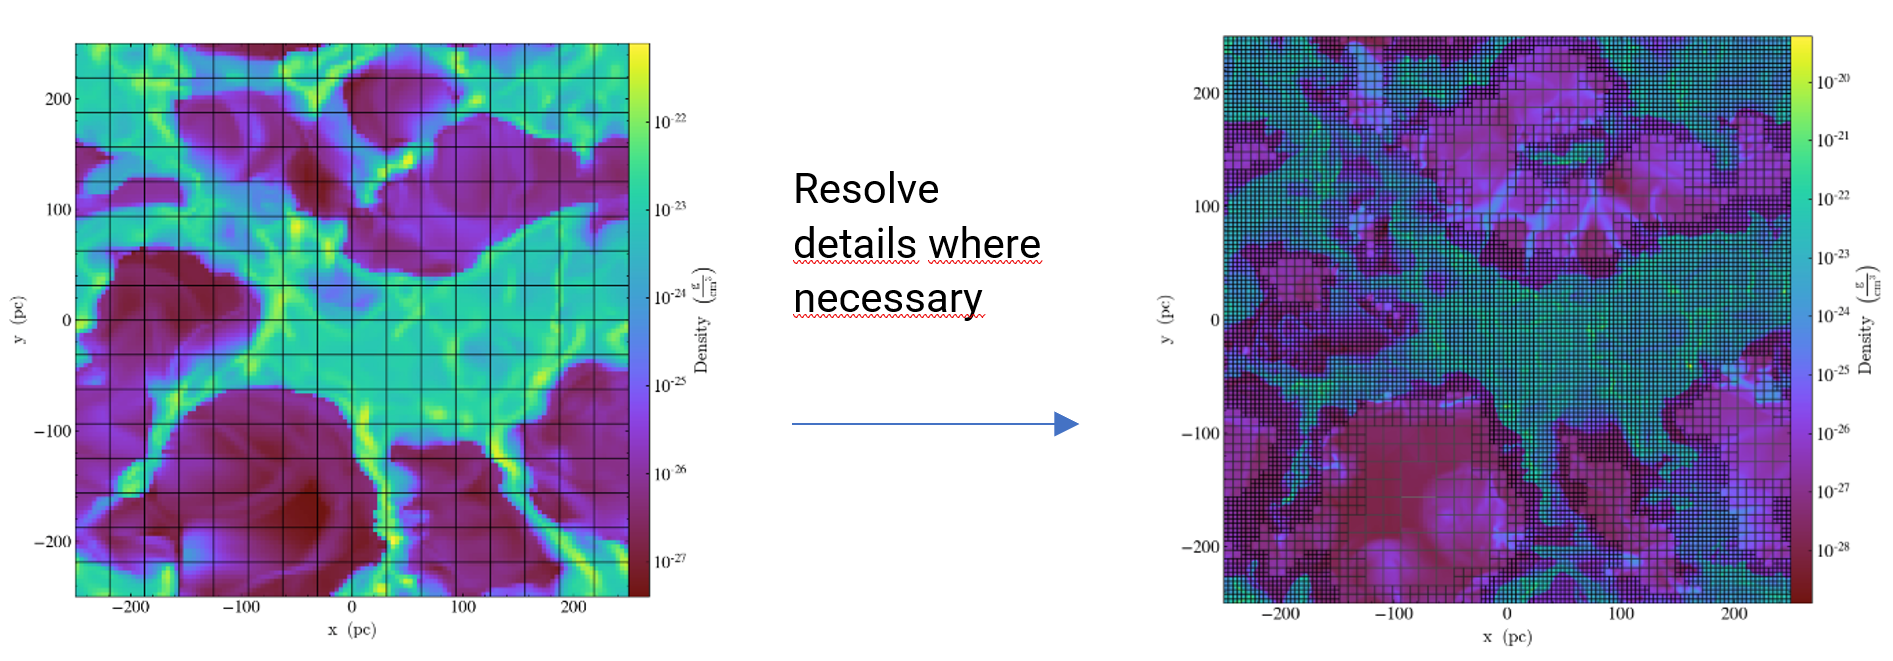
\includegraphics[width=0.8\textwidth]{figures/adaptive_mesh.png}\hfill
  \caption{Grid refinement for interstellar medium.}
  \label{fig:refined_grid}
\end{figure}

\begin{figure}[!htb]
    \centering
    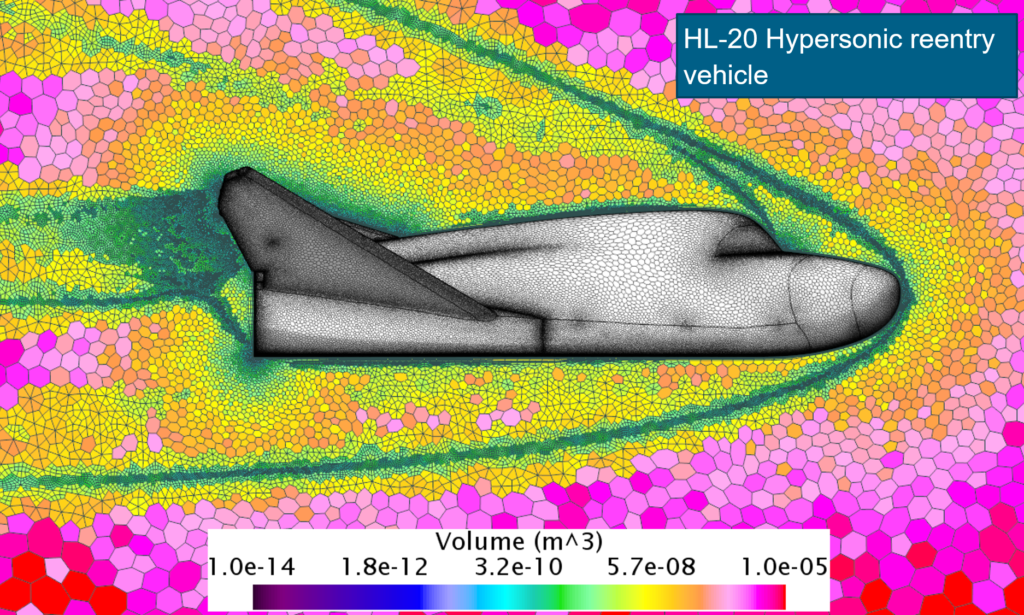
\includegraphics[width=0.8\textwidth]{figures/jet_refined.png}\hfill
    \caption{Adaptive mesh for the simulation of a supersonic jet.}
    \label{fig:grid_jet}
\end{figure}

\greybox{\textbf{How to distribute the simulation onto processes?:} A simple approach is to give
all processes the same number of cells with domains chosen to limit communication (/ minimize
to overall borderlenght) and cell-size chosen e.g. to have the roughly the same number of particles
(equal memory distribution over cells). \textcolor{red1}{Problems:}
\begin{itemize}
    \item with increasing distribution increases the necessary communication, giving us a limit
    until which parallelization makes sense (beyond this further parallelization does not yield
    better performance)
    \item in the simple \textit{memory balanced} approach, we neglect that different cells can have 
    different costs (see physical load balancing below)
\end{itemize}}

\yellowbox{\textbf{Local timesteps | physics load balancing:} Small cells interact on smaller time scales so
they require smaller timesteps (as before with the CFL criterion), \textcolor{red1}{so more iterations
to cover the same time as for larger cells are necessary - so the workload for smaller cells is higher}.
\textcolor{green1}{Decompose the domain according to work for more balanced tasks.}}

\subsubsubsection{Inclusion of long-range forces | long range forces vs. parallelization}
In hydrodynamics interactions are short-range, information travels
\textit{one cell at a time}, a cell might be updated only based on
its neighbors. Therefore, if we divide the domain into subdomains to distribute
them onto processes, \textcolor{green1}{a padding of only one (communicated) guard cell is sufficient
for pure hydrodynamics} (for a \textit{three-point-stencil}).
\redbox{\textbf{But gravity is an instantanous long-range interaction:}
\begin{itemize}
    \item all cells are interdependent $\rightarrow$ all processes need to communicate (not only those handling neighboring regions)
    \item so practically every process while only updating its subdomain would need to have all particles in memory
\end{itemize}}
\idea{While each process also needs distant information it must not be highly resolved - we can reduce
communication by all processes working on a shared tree (possibly managed by one MPI rank / \textit{arced RWLock in Rust}). For a distant group under small opening angle
a single process must only retrieve the respective center-of-mass force, limiting communication.}

So we can do (magneto)-hydrodynamics based on local information transfer and reduce the communication
of (self)-gravitation via a shared tree structure.

\subsection{Scaling of the processing time with increasing parallelism and Ahmdal's law}
Concurrency is the partial-decomposability of a problem. The maximum speed-up gained
from parallelization (the ratio of execution time with and wihtout parallization $= t_1 \slash t_N$)
is limited by the fraction of the problem, that is not decomposable.

\paragraph*{Strong scaling} Consider a fixed problem size. When using multiple processes
the ideal speedup would be $\propto N_{proc}$ as $t_{N_{proc}} = t_{1} \slash N_{proc}$. The not-parallelizable
part gives an upper limit for the speedup (\textbf{Ahmdal's law})
\begin{equation}
    \begin{gathered}
        \text{speedup } = \frac{1}{s + \frac{p}{N_{proc}}}, \quad \text{proportion of execution time of parallelizable part } p \\
        \text{proportion of execution time of serial part } s
    \end{gathered}
\end{equation}
The higher the non parallelizable part, the worse the scaling, see
figure \ref{fig:ahmdal}. Strong scaling is measured by how the
computational time increases with the number of processes for
a constant job size.

\paragraph*{Weak scaling} Here we consider the amount of work done
for a scaled problem size. In Gustafson's law it is assumed that the
parallel part scales linearly with the processes, while the serial
part does not increase, $\text{speedup } = s + pN$. Weak scaling
is tested by increasing job size and number of processes.

\note{In real application the overhead of parallelization increases
with problem size, reducing the speedup.}

\subsection{Examples of parallel algorithms}
\begin{itemize}
    \item sorting numbers in parallel
    \begin{itemize}
        \item even-odd-sort: while in (stupid) bubble sort we go through the list and consecutively swap, so $[72964] \rightarrow [27649]$ after one
        run (and we might need $N$ of them), we can also make this independent by considering only consecutive pairs in each step, so
        $[72,96,4] \rightarrow [27,69,4]$ (can be done in parallel), then $[2,76,94] \rightarrow [2,67,49]$
        \item parallel merge sort: sort chunks of the list in parallel, then merge
    \end{itemize}
    \item parallel FFT: In a 3D FFT problem, we can split the domain into 2D slices and start by performing FFTs along their axis and after a transposed
    composition a final FFT along the missing axis, for detials see \cite{jagode06}.
\end{itemize}


\subsection{Notes on sheduling}
\problem{If tasks (a sequence of commands executed by a thread) need totally different computation times,
the slowest task is the bottleneck for subsequent merging. For instance in a Milky Way SPH simulation
where we would want to do time-steps on the order of $10^5$ years, the bottleneck are cells
with supernovae for which we would need to do mutliple time-steps on the order of $10^3$ years.}

\paragraph*{Task based scheduling:} One approach is to estimate the cost of tasks and distribute work wisely accordingly.
Another is work having a worker pool with work stealing. Work is distributed to workers
but if one finishes early, it can steal work from another worker and not just wait,
which might be more or less feasable depending on the problem.

\paragraph*{Async:} Asynchronous runtimes can allow us to write code similar as in a non-parallel setting 
while managing the distribution of work - we specify
when we need what results (async / await).


